% Upload fig_completed_acd_relations.pdf; requires graphicx.
\begin{figure*}[t]
  \centering
  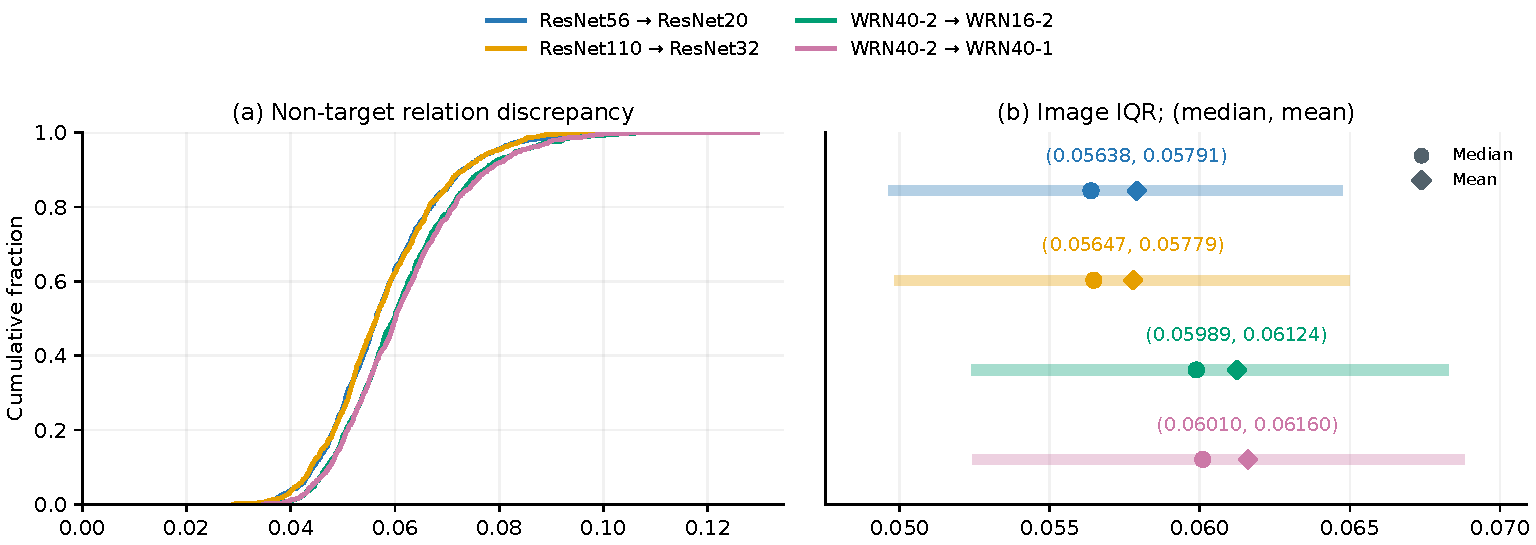
\includegraphics[width=.9\textwidth]{fig_completed_acd_relations.pdf}
  \caption{\textbf{Non-target relation discrepancies of completed ACI+SICD models.}
  Four epoch-240, seed-3201 models are evaluated on the same first 1,024
  official CIFAR-100 test images. Teacher and student logits are independently
  standardized over all classes before non-target conditioning at $T=4$.
  (a) Empirical cumulative distributions of conditional total variation.
  (b) Per-model medians (circles), means (diamonds), and image interquartile
  ranges (segments). These are image-level distributions for one trained
  seed per pair, not confidence intervals over independent training runs.
  Models use the complete conditional objective with gradient-strength
  matching and no ETF initialization. No matched baseline is included;
  across-pair differences do not establish relative method effectiveness.}
  \label{fig:completed_acd_relations}
\end{figure*}
